\chapter{Asking Entrepreneurs How They Got Rich (San Antonio)}

This lecture is not a theorem-driven blackboard talk. It is a field notebook on wealth, built out of short interviews, and its mathematical payload comes from the way repeated claims harden into mechanisms. We begin with headline numbers, move into staged growth, reputation, perseverance, land, craft, and finally a layered business model connecting real estate, Airbnb, Turo, and exotic cars. The safest way to read it is to separate anecdote, claim, and mechanism, and to formalize only what the transcript actually supports.

\section{Opening Montage: Results Before Theory}

The lecture opens by refusing abstraction. We are first given income claims and only afterward the question of how those claims were produced. That order matters. The transcript is teaching us to ask for a mechanism only after we know that somebody has actually operated at scale.

\begin{align}
G_{\text{peak},1} &\approx \$1{,}000{,}000,\\
G_{\text{peak},2} &> \$500{,}000,\\
W_{\text{developer}} &\approx \$15\text{M}-\$20\text{M}.
\end{align}

These are not yet conclusions. They are boundary conditions. The lecture uses them to justify a search for rules that survive across industries.

\paragraph{Claim.} Wealth is introduced here as something observable through reported peak income, net worth, and scale.

\paragraph{Mechanism.} The chapter should therefore proceed by asking, each time, what operating rule converts a one-line credential into a repeatable structure.

\section{Crawl, Walk, Run: Scaling Without Self-Destruction}

The first full interview belongs to an operator who has moved through wealth management, company leadership, and construction. The sequence is important: breadth first, then the rule of scale, then the warning against over-leverage, and only then the personal claim that a stable home life supports business life.

The rule is stated in plain language, but we can write it in a compact form:
\begin{equation}
\text{crawl} \to \text{walk} \to \text{run},
\qquad
\text{expertise} \prec \text{leverage}.
\end{equation}

What this means in the lecture is not that all firms must move slowly. It means that the order of operations matters. One learns the industry, becomes expert in it, and only then tolerates more balance-sheet risk.

\subsection{Question \& Answer}

\paragraph{Question.} How do we scale a business without blowing ourselves up?

\paragraph{Answer.} The lecture's answer is staged expansion. If we accelerate before we understand the business, then leverage amplifies ignorance. If we build expertise first, then later scale is attached to a recoverable operating process rather than to optimism alone.

\paragraph{Mechanism.} The hidden variable is recoverability. Running too fast is dangerous not because speed is immoral, but because it makes it harder to pick oneself back up after a mistake.

A second point is folded into this first answer. The speaker treats marriage and personal stability as financially relevant, not sentimental decoration. The lecture therefore refuses a sharp line between professional scaling and the conditions that make disciplined action sustainable over time.

\section{Character, Perseverance, and the Labor Market}

From the first operator the lecture pivots into a broader rule: every day is an interview, every day is a resume. The point is that reputation is accumulated continuously and not just during a formal hiring event. The lecture does not offer a literal formula here, so we keep the claim conceptual: conduct is a repeated input into future opportunity.

The caricature intermission then resets the rhythm, and the next entrepreneur enters through bioinformatics. Again the lecture moves in the same order: industry, recent exit, then advice. The core claim is that perseverance is underappreciated because everybody experiences friction, and growth comes through that friction rather than around it.

\paragraph{Claim.} The important difference is not merely intelligence or even novelty. It is the ability to continue when the local evidence looks unfavorable.

\paragraph{Mechanism.} Friction does not automatically imply failure. In the lecture it is the ordinary medium through which growth is purchased.

The beat closes on AI, and the lecturer sharpens the point by making it operational rather than futuristic. The danger is not an abstract machine replacing us; it is another worker learning how to use the machine more effectively than we do.

\subsection{Question \& Answer}

\paragraph{Question.} What separates the person who survives early business adversity from the person who exits too soon?

\paragraph{Answer.} The transcript gives a two-part answer. First, we stick with the work through friction. Second, we update our tool set. In this case the contemporary tool set includes AI, and the lecture's warning is that adaptation is competitive.

\section{Real Estate as Scarcity, Tax Treatment, and Risk}

The Westin interview is where the lecture turns from personal advice to capital allocation. We are told about approximately million-dollar annual earnings and a net worth in the range of \$15M to \$20M, and then the central question is posed: where should new money go if one wishes to compound it?

The answer is land. The lecture's logic is not mystical. It is a chain of scarcity, cost, and optionality:
\begin{equation}
\text{fixed supply of land} + \text{rising development cost}
\;\Longrightarrow\;
\text{scarcity value with development optionality}.
\end{equation}

A second part of the mechanism concerns carrying cost:
\begin{equation}
\text{carry cost} = \text{tax burden} + \text{other holding costs},
\qquad
\text{agricultural use} \Rightarrow \text{smaller tax burden}.
\end{equation}

The lecture does not supply tax rates, and so we do not invent them. The point is structural: if a piece of land can be held with a lighter tax load, then the investor buys time. That time preserves the option to develop or sell later.

\subsection{Question \& Answer}

\paragraph{Question.} Why land, and why take the plunge rather than wait for certainty?

\paragraph{Answer.} The lecture gives two answers. Land is attractive because nobody is making more of it, and because it can later be developed or sold into a higher-cost environment. Risk is then justified not as thrill-seeking but as a learning device: even failure leaves us with information and experience we did not have before.

\begin{remark}
This is a mechanism-heavy section with limited numeric detail. The final notes should preserve the causal sequence without pretending that the lecture derived a formal real-estate pricing model.
\end{remark}

\section{Long-Horizon Craft, Output, and Lifestyle Choice}

The caricature artist returns and slows the lecture down. Here the point is not scaling a balance sheet but sustaining a craft. We are told about roughly \(35\) years of work, about friendliness and generosity in the public, and about the artist's original ambition to be like Picasso. The dream is not fully realized in its youthful form, but the lecture treats the actual career as a serious economic achievement.

The most striking quantitative statement is cumulative:
\begin{equation}
N_{\text{drawn}} \approx 5\times 10^5.
\end{equation}

A cautious average-rate calculation makes the lecture's point vivid:
\begin{align}
T &\approx 35 \text{ years},\\
\bar N_{\text{year}} &\approx \frac{N_{\text{drawn}}}{T}
\approx \frac{500{,}000}{35}
\approx 1.43\times 10^4 \text{ drawings/year}.
\end{align}

This is not a claim of uniform yearly output. It is a way of seeing what persistence looks like when accumulated over decades.

The architect interview that follows extends the same theme in a different key. The range of annual income is lower than the hotel developer's or the later Airbnb operator's, but the advice is sharp: choose based on the lifestyle one wants to live. The lecture is telling us that the optimization problem is not one-dimensional. Income matters, but so does fit between work and life.

\subsection{Question \& Answer}

\paragraph{Question.} What does persistence buy us, if not immediate fame?

\paragraph{Answer.} In this lecture it buys cumulative output, professional competence, and credibility. We may not receive the exact youthful fantasy, but repeated work over long horizons can still build a real economic and human position.

\section{From Passion to Platform: Real Estate, Airbnb, and the First Deal}

The final movement returns to the R8 owner, and now the lecture begins to integrate the earlier motifs. The advice starts with consistency and discipline, but it quickly turns operational: real estate was the first major investment, the reported gross peak was approximately \$1.3M, and the path to wealth begins by finding something one cares enough about to study seriously and duplicate.

The duplication rule is stated almost like a map:
\begin{equation}
\text{research} \to \text{first deal} \to \text{duplication at scale}.
\end{equation}

We are then given an approximate portfolio size:
\begin{equation}
N_{\text{properties}} \approx 38 - 40.
\end{equation}

Humility reappears as a growth condition. In the lecture's language, staying humble keeps learning open, and open learning prevents early success from hardening into arrogance.

\subsection{Question \& Answer}

\paragraph{Question.} If we start with zero properties and zero rentals, what is the first step?

\paragraph{Answer.} Research. The transcript is very explicit about the order. First inspect the city. Then inspect the exact area. Then inspect the platform itself, here Airbnb. Only after that do we move toward controlling a unit and testing the offer in a real market.

We can make the gross annualization example explicit. The lecture says that a first property might gross roughly \$3{,}000 to \$5{,}500 per month. If we annualize that range,
\begin{align}
G_{\text{month, property}} &\approx \$3{,}000 - \$5{,}500,\\
G_{\text{year, property}} &\approx 12\,G_{\text{month, property}},\\
G_{\text{year, property}} &\approx \$36{,}000 - \$66{,}000.
\end{align}

This is a gross calculation only. The lecture does not subtract vacancy, furnishing, debt service, maintenance, cleaning, or platform fees, so neither do we.

\begin{figure}
\centering
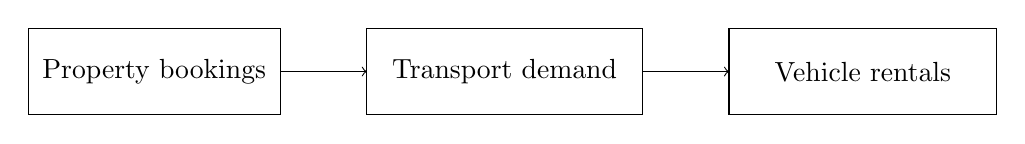
\begin{tikzpicture}
\draw (0,0) rectangle (3.2,1.1);
\draw (4.3,0) rectangle (7.8,1.1);
\draw (8.9,0) rectangle (12.3,1.1);
\node at (1.6,0.55) {Property bookings};
\node at (6.05,0.55) {Transport demand};
\node at (10.6,0.55) {Vehicle rentals};
\draw[->] (3.2,0.55) -- (4.3,0.55);
\draw[->] (7.8,0.55) -- (8.9,0.55);
\end{tikzpicture}
\end{figure}

This figure is not a reconstruction of a board drawing. It is a cleaned statement of the lecture's business logic: one layer creates demand for the next.

\section{Layered Cash Flow: Exotic Cars and Unit Economics}

Only at this point does the R8 stop being a teaser and become a business object. The lecture says that the car business grew out of the property business. Guests book a stay, then need transportation, and from there the operator adds regular cars and exotic cars. The point is not glamour for its own sake; the point is service layering.

The fleet size is reported as approximately
\begin{equation}
N_{\text{fleet}} \approx 6.
\end{equation}

The lecture then gives its clearest quantitative material:
\begin{align}
G_{\text{month, exotic}} &\approx \$8{,}000 - \$10{,}000 \text{ on some cars},\\
r_{\text{R8}} &\approx \$600 - \$700 \text{ per day}.
\end{align}

A useful consistency check is
\begin{equation}
G_{\text{month, car}} \approx r_{\text{day}}\,d_{\text{booked}},
\end{equation}
so that
\begin{equation}
d_{\text{booked}} \approx \frac{G_{\text{month, car}}}{r_{\text{day}}}.
\end{equation}

If we insert the quoted ranges only as a rough example, we obtain
\begin{equation}
d_{\text{booked}} \approx \frac{\$8{,}000 - \$10{,}000}{\$600 - \$700}
\approx 11.4 - 16.7 \text{ booked days/month}.
\end{equation}

This is not a lecture-stated occupancy derivation, and it should be read cautiously. The monthly gross figure is said to apply to some cars, not necessarily the R8 alone. Still, the estimate shows why the speaker can say that weekend bookings matter so much.

\subsection{Question \& Answer}

\paragraph{Question.} How do we get started in exotic car rentals without treating the business like fantasy?

\paragraph{Answer.} The lecture gives a structural answer. We begin by forming the LLC, learning how to place vehicles inside it, and building or using the relevant credit channels. Some manufacturers or dealers may be more flexible than others. Down payment and income both matter. Most importantly, the exotic layer is best understood as something added on top of an existing business rather than as a first and only foundation.

In compact form, the lecture's startup chain is
\begin{equation}
\text{LLC} + \text{credit/funding} \to \text{vehicle acquisition} \to \text{rental revenue}.
\end{equation}

\begin{remark}
The transcript prints ``RA'' in several places, but the context makes clear that the intended car is the Audi R8. The notes should preserve that normalization while remembering that the underlying transcript is noisy.
\end{remark}

\section{Summary}

The lecture begins with flashy numbers and ends by stripping the flash away. Across operators, developers, artists, founders, and the R8 owner, the same few rules repeat: scale in stages, do not lever ignorance, treat reputation as cumulative, persist through friction, buy time where taxes and holding structure allow it, research before committing capital, and build new revenue layers on top of proven ones.

What makes the lecture useful is that it keeps moving from result to mechanism. A million-dollar year, a \$15M--\$20M net worth, half a million drawings, \(38\)--\(40\) properties, six cars, \$600--\$700 per day for an R8: these numbers are not the lesson by themselves. The lesson is the machinery underneath them. We are meant to leave with a sequence of operational rules, not with admiration alone.